% !TEX program = xelatex
\documentclass[withoutpreface]{cumcmthesis}

\usepackage{tikz}
\usepackage{pythonhighlight}
\usetikzlibrary{positioning, arrows.meta, calc, shapes.geometric}
\captionsetup{font=small}
\newtheorem{proposition}{命题}

\title{这里是标题}

\begin{document}

\maketitle

\begin{abstract}
这里是摘要
\keywords{这里是关键词}
\end{abstract}

% ==================== 问题重述 ====================
\section{问题重述}

\subsection{问题背景}

中国天眼——500米口径球面射电望远镜（Five-hundred-meter Aperture Spherical radio Telescope，简称FAST），是我国自主建造的目前世界上单口径最大、灵敏度最高的射电望远镜。其主动反射面由主索网、反射面板、下拉索与促动器等构成一个可调节球面：主索网按短程线三角网格布置并支承反射面板，每个主索节点经一根长度固定的下拉索与地表促动器相连，促动器沿基准球面径向伸缩即可牵引主索节点变位，从而改变反射面的整体形状。

主动反射面有基准态与工作态两种状态：基准态为半径约$300\,\mathrm{m}$、口径$500\,\mathrm{m}$的球面（基准球面，球心记为$C$）；工作态则被调节为口径$300\,\mathrm{m}$的近似旋转抛物面（工作抛物面）。馈源舱接收平面中心只能在与基准球面同心、半径差为$F=0.466R$的焦面上移动，其有效接收区域为直径$1\,\mathrm{m}$的中心圆盘。当观测方向为天体目标$S$时，馈源舱中心移至直线$SC$与焦面的交点$P$，并通过调节部分反射面板形成以$SC$为对称轴、$P$为焦点的近似旋转抛物面，将平行入射的电磁波汇聚至馈源舱。本赛题的核心任务，即在此调节机制约束下确定理想抛物面，并通过调节促动器的径向伸缩量使反射面尽量贴近该理想抛物面，以获得最佳接收效果。FAST观测时的剖面示意如图~\ref{fig:fast_profile}所示。

\begin{figure}[htbp]
    \centering
    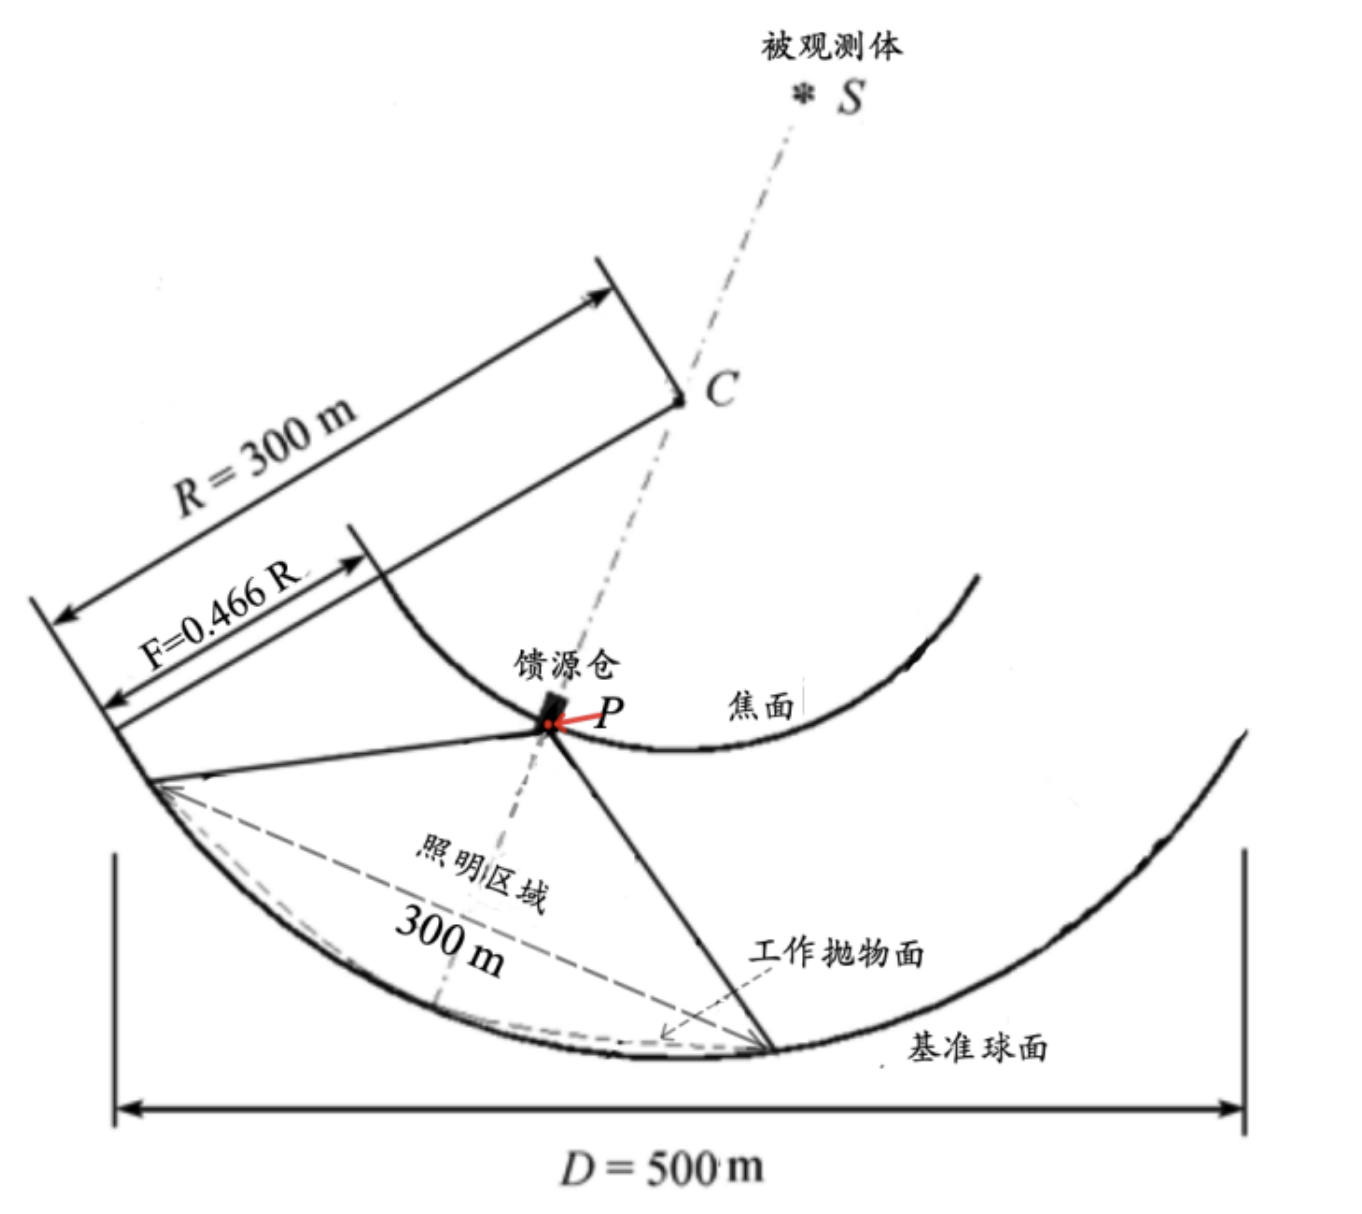
\includegraphics[width=0.65\textwidth]{../figures/FAST_cross-sectional_schematic.png}
    \caption{FAST观测剖面示意图} \label{fig:fast_profile}
\end{figure}

\subsection{问题提出}

根据上述背景及附录所给参数，本文需要建立模型解决以下三个问题：

\textbf{问题一}：当待观测天体$S$位于基准球面正上方，即方位角$\alpha=0^{\circ}$、仰角$\beta=90^{\circ}$时，结合考虑反射面板调节因素，确定理想抛物面。

\textbf{问题二}：当待观测天体$S$位于$\alpha=36.795^{\circ}$、$\beta=78.169^{\circ}$时，确定理想抛物面；建立反射面板调节模型，调节相关促动器的伸缩量，使反射面尽量贴近该理想抛物面。将理想抛物面的顶点坐标，以及调节后反射面$300\,\mathrm{m}$口径内的主索节点编号、位置坐标、各促动器的伸缩量等结果，按附件4规定的格式保存在\texttt{result.xlsx}文件中。

\textbf{问题三}：基于第2问的反射面调节方案，计算调节后馈源舱的接收比，即馈源舱有效区域接收到的反射信号与$300\,\mathrm{m}$口径内反射面的反射信号之比，并与基准反射球面的接收比作比较。

% ==================== 问题分析 ====================
\section{问题分析}

\subsection{问题一分析}

问题一要求在天体$S$位于基准球面正上方（$\alpha=0^{\circ}$，$\beta=90^{\circ}$）时确定理想抛物面。此时抛物面的对称轴沿$z$轴正方向，馈源舱位于轴线上方。解决此问题的关键步骤为：首先建立馈源舱（焦点）的位置模型，利用焦径比$F/R=0.466$确定焦点坐标；然后根据抛物面的几何定义——抛物面上任意一点到焦点的距离等于该点到准线的距离——推导出理想抛物面的解析方程；最后代入$\alpha=0^{\circ}$、$\beta=90^{\circ}$的特殊条件，得到该情形下的具体抛物面方程及其顶点坐标。

\subsection{问题二分析}


\subsection{问题三分析}


% ==================== 问题假设 ====================
\section{问题假设}

\begin{description}
\item[1. ] 反射面板为理想刚性平面，不考虑其自身弹性变形，调节后面板形状严格由三个顶点（主索节点）决定。
\item[2. ] 电磁波信号及反射信号均视为直线传播，不考虑大气折射等影响。
\item[3. ] 主索节点调节后，相邻节点之间的距离变化幅度不超过$0.07\%$，即可视为索长近似不变。
\item[4. ] 反射面板上的小圆孔直径远小于所观测天体电磁波的波长，不影响反射效果，可视为无孔面板。
\item[5. ] 促动器沿基准球面径向安装，其伸缩方向严格沿径向指向球心，伸缩范围为$-0.6\sim+0.6\,\mathrm{m}$。
\item[6. ] 将主索节点坐标视为对应的反射面板顶点坐标，即面板顶点与主索节点重合。
\item[7. ] 基准态下所有主索节点均严格位于基准球面上。
\end{description}

% ==================== 符号说明 ====================
\section{符号说明}

\begin{longtable}{c p{4.2cm} c | c p{4.2cm} c}
\toprule
符号 & 说明 & 单位 & 符号 & 说明 & 单位 \\
\midrule
\endfirsthead
\toprule
符号 & 说明 & 单位 & 符号 & 说明 & 单位 \\
\midrule
\endhead
\bottomrule
\endfoot
\bottomrule
\endlastfoot
$R$ & 基准球面半径（$\approx300$） & $\mathrm{m}$ & $F$ & 焦距，$F=0.466R$ & $\mathrm{m}$ \\
$C$ & 基准球面球心（坐标原点） & --- & $D$ & 基准球面口径（$500$） & $\mathrm{m}$ \\
$\alpha$ & 天体方位角 & $^{\circ}$ & $\beta$ & 天体仰角 & $^{\circ}$ \\
$\mathbf{n}$ & 抛物面轴线方向向量 & --- & $F/R$ & 焦径比（$0.466$） & --- \\
$Q$ & 馈源舱（抛物面焦点） & --- & $\vec{OQ}$ & 馈源舱位置向量 & $\mathrm{m}$ \\
$M(x,y,z)$ & 抛物面上任意一点 & $\mathrm{m}$ & $f$ & 抛物面焦距，$f=0.466R$ & $\mathrm{m}$ \\
$a,b,c$ & 轴向量$\mathbf{n}$的分量 & --- & $V$ & 抛物面顶点 & --- \\
\end{longtable}

% ==================== 问题一 ====================
\section{问题一：理想抛物面的确定}

\subsection{模型建立}

\subsubsection{馈源舱（焦点）位置模型}

设抛物面轴线方向向量为$\mathbf{n}$，由天体方位角$\alpha$和仰角$\beta$可得：
\begin{equation}
\mathbf{n} = (\cos\beta\cos\alpha,\;\cos\beta\sin\alpha,\;\sin\beta)
\end{equation}

记$a=\cos\beta\cos\alpha$，$b=\cos\beta\sin\alpha$，$c=\sin\beta$，则$\mathbf{n}=(a,b,c)$。

馈源舱$Q$位于抛物面轴线上，且为抛物面的焦点。由题目条件，馈源舱接收平面中心$P$位于焦面上，焦面半径$R-F=R-0.466R=0.534R$。因此馈源舱的位置向量为：
\begin{equation}
\vec{OQ} = -0.534R\,\mathbf{n}
\end{equation}

即焦点$Q$的坐标为：
\begin{equation}
Q = (-0.534Ra,\;-0.534Rb,\;-0.534Rc)
\end{equation}

\subsubsection{理想抛物面模型}

由抛物面的几何定义，抛物面上任意一点$M(x,y,z)$到焦点$Q$的距离等于该点沿轴线方向到准线的距离，即：
\begin{equation}
\left|\vec{OM}-\vec{OQ}\right| = (\vec{OM}-\vec{OQ})\cdot\mathbf{n} + 2F
\end{equation}

将$\vec{OM}=(x,y,z)$、$\vec{OQ}=-0.534R\,\mathbf{n}$代入上式，得：
\begin{multline}
(x+0.534Ra)^{2} + (y+0.534Rb)^{2} + (z+0.534Rc)^{2} \\
= (ax+by+cz+0.534R+2F)^{2}
\end{multline}

其中$F=0.466R$为焦距。

\subsection{求解过程}

当待观测天体$S$位于基准球面正上方时，$\alpha=0^{\circ}$，$\beta=90^{\circ}$，代入方向向量得：
\begin{equation}
a = \cos 90^{\circ}\cos 0^{\circ} = 0,\quad
b = \cos 90^{\circ}\sin 0^{\circ} = 0,\quad
c = \sin 90^{\circ} = 1
\end{equation}

即轴线方向为$\mathbf{n}=(0,0,1)$，抛物面以$z$轴为对称轴。将上述分量代入抛物面方程~(5)：
\begin{equation}
x^{2}+y^{2}+(z+0.534R)^{2} = (z+0.534R+2F)^{2}
\end{equation}

记$u=z+0.534R$，则上式化为：
\begin{equation}
x^{2}+y^{2}+u^{2} = (u+2F)^{2}
\end{equation}

展开右端：
\begin{equation}
x^{2}+y^{2}+u^{2} = u^{2}+4Fu+4F^{2}
\end{equation}

化简得：
\begin{equation}
x^{2}+y^{2} = 4Fu+4F^{2} = 4F(u+F) = 4F(z+0.534R+F)
\end{equation}

将$F=0.466R$代入$0.534R+F=0.534R+0.466R=R$，故：
\begin{equation}
\boxed{x^{2}+y^{2} = 4F(z+R)}
\end{equation}

此即问题一的理想抛物面方程，是以$z$轴为对称轴、开口向$z$负方向的旋转抛物面。

抛物面顶点坐标为$V(0,\,0,\,-R)$，即$(0,\,0,\,-300)$，恰与基准球面的最低点（南极）重合。

代入$R=300\,\mathrm{m}$，$F=0.466\times300=139.8\,\mathrm{m}$，抛物面方程为：
\begin{equation}
x^{2}+y^{2} = 559.2\,(z+300)
\end{equation}

\subsection{求解结果}

问题一的求解结果如表~\ref{tab:q1_result}所示。

\begin{longtable}{lc}
\caption{问题一求解结果} \label{tab:q1_result} \\
\toprule
指标 & 数值 \\
\midrule
\endfirsthead
\toprule
指标 & 数值 \\
\midrule
\endhead
\bottomrule
\endfoot
\bottomrule
\endlastfoot

\end{longtable}


% ==================== 问题二 ====================
\section{问题二}

% ==================== 问题三 ====================
\section{问题三}

% ==================== 结果分析与检验 ====================
\section{结果分析与检验}


% ==================== 模型评价与推广 ====================
\section{模型评价与推广}

\subsection{模型优点}

\begin{itemize}
\item \textbf{}：
\end{itemize}

\subsection{模型不足}


\subsection{模型推广}

% ==================== AI工具使用说明 ====================
\section{AI工具使用说明}

本作品在撰写过程中使用了以下AI工具辅助完成部分工作：

\begin{itemize}
    \item \textbf{DeepSeek网页端}（DeepSeek-V4-Flash/Pro）：
    \item \textbf{MiMo Code}（MiMo-v2.5-Pro）：
    \item \textbf{TRAE}（字节跳动AI编程助手）：
    \item \textbf{Codex}（OpenAI代码生成模型）：
\end{itemize}

\textbf{人工修改与质量保证}：

% ==================== 参考文献 ====================
\begin{thebibliography}{99}

\end{thebibliography}

% ==================== 附录 ====================
\appendix
\section{附录：核心代码}

本节展示求解模型的核心代码。完整代码及数据文件详见随附电子材料。


\end{document}









